\documentclass[10pt]{article}

\usepackage[english]{babel}
\usepackage[utf8]{inputenc}
\usepackage[T1]{fontenc}
\usepackage[margin=0.65in,top=0.75in,bottom=0.75in]{geometry}
\usepackage{amsmath, amssymb, mathtools}
\usepackage{physics}
\usepackage{graphicx}
\usepackage{enumitem}
\usepackage{fancyhdr}
\usepackage[most]{tcolorbox}
\usepackage[colorlinks=true, allcolors=blue]{hyperref}
\usepackage{titlesec}
\usepackage{multicol}

\graphicspath{{figures/}}
\titlespacing*{\section}{0pt}{5pt}{2pt}
\titleformat*{\section}{\normalsize\bfseries}
\setlength{\parskip}{2pt}
\setlength{\parindent}{0pt}
\setlength{\abovedisplayskip}{4pt}
\setlength{\belowdisplayskip}{4pt}
\setlength{\abovedisplayshortskip}{2pt}
\setlength{\belowdisplayshortskip}{2pt}
\setlist{itemsep=1pt,topsep=2pt,leftmargin=*}

\providecommand{\erf}{\operatorname{erf}}
\newcommand{\lth}{\lambda_{\mathrm{th}}}
\newcommand{\Cq}{C_v^{\mathrm{q}}}
\newcommand{\Ccl}{C_v^{\mathrm{cl}}}
\newcommand{\kB}{k_{B}}

\newtcolorbox{keybox}{colback=lightgray!15, colframe=black, arc=2pt, boxrule=0.6pt,
  left=1.5mm, right=1.5mm, top=0.8mm, bottom=0.8mm}

\pagestyle{fancy}
\fancyhf{}
\lhead{\small 00540367: Research Project 1}
\rhead{\small Technion - IIT}
\lfoot{\small Spring 2026 | Semester 6}
\rfoot{\small Page \thepage}
\renewcommand{\headrulewidth}{0.4pt}
\renewcommand{\footrulewidth}{0.4pt}

\begin{document}

\begin{center}
{\large\bfseries An exactly solvable case of $\Cq>\Ccl$: a P\"oschl--Teller well in a box}\\[1mm]
{\small Nadav Jean \quad$\cdot$\quad summary for the supervisor meeting, 28.10.2026\quad$\cdot$\quad derivations in \texttt{PT\_Box\_Derivation.pdf}}
\end{center}

\section{The system}
A particle of mass $m$ in a P\"oschl--Teller well placed in the middle of an infinite square well of length $L$:
\begin{equation}
V(x)=-\frac{\hbar^2}{2m}\,\alpha^2\,\frac{\lambda(\lambda-1)}{\cosh^2(\alpha x)}
\;\xrightarrow{\;\lambda=2\;}\;
-\frac{\hbar^2\alpha^2}{m}\,\frac{1}{\cosh^2(\alpha x)}\quad(|x|<L/2),\qquad V=+\infty\quad(|x|\ge L/2).
\label{eq:V}
\end{equation}
The well is the ``modified P\"oschl--Teller well'' written exactly as in Table~I of Deffner, Jarzynski and del Campo~\cite{deffner}, who take it from Fl\"ugge~\cite{flugge}. It has depth $\hbar^2\alpha^2/m$ and width $\sim1/\alpha$. We use $\lambda=2$, the simplest \emph{reflectionless} case: a wave crosses the well without any reflection~\cite{LL,lekner}. That single property is what makes every result below exact. Only two numbers matter: $\alpha L$ (box length in well widths) and $\kB T/(\hbar^2\alpha^2/2m)$.

\begin{figure}[h]
\centering
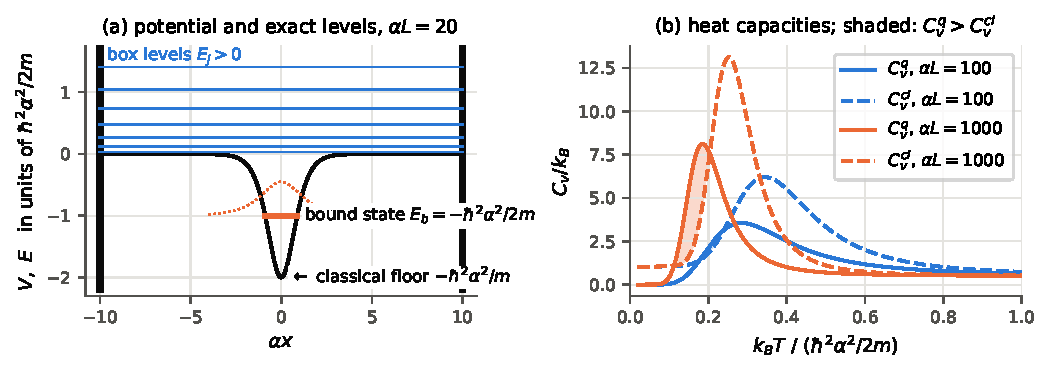
\includegraphics[width=0.86\textwidth]{fig_summary.pdf}\vspace{-2mm}
\caption{\small (a) The potential (black), the box levels (blue) and the single bound state (orange, with its wavefunction $\propto1/\cosh\alpha x$ dotted), for $\alpha L=20$. (b) $\Cq$ (solid) and $\Ccl$ (dashed) for $\alpha L=100$ and $1000$; shaded where $\Cq>\Ccl$.}
\label{fig:1}
\end{figure}\vspace{-3mm}

\section{Energy levels (exact)}
\begin{itemize}
\item \textbf{One bound state, halfway up the well}~\cite{LL}: $E_b=-\hbar^2\alpha^2/2m$, with wavefunction $\propto1/\cosh(\alpha x)$. The other half of the depth is zero-point energy.
\item \textbf{Box levels}~\cite{lekner,CKS}: $E_j=\hbar^2k_j^2/2m$, $j=1,2,\dots$, with
\begin{equation}
k_jL=j\pi+2\arctan\!\left(\frac{k_j}{\alpha}\right).
\label{eq:levels}
\end{equation}
\end{itemize}
Both hold up to corrections of order $e^{-\alpha L}$ (the exact finite-$L$ equations are in the derivation). \emph{Heuristic:} without the well, $k_jL=j\pi$. Far from the well, all the well does to a wave is shift its phase by $2\arctan(k/\alpha)$, which pushes every box level up by less than one spacing. As $k\to\infty$ the shift tends to $\pi$, so level $j$ moves up to where level $j+1$ of the empty box was: exactly one state has left the continuum, and it is the bound state (Levinson's theorem~\cite{levinson}).

\section{Quantum heat capacity}
$Z_q=e^{-\beta E_b}+\sum_je^{-\beta E_j}$ and $\Cq=\kB\beta^2\,\mathrm{Var}(E)$~\cite{pathria}. Writing the sum over $j$ as an integral over $k$ (Poisson summation~\cite{dlmf}), with the level density $\dd j/\dd k$ read off Eq.~\eqref{eq:levels} (the Beth--Uhlenbeck idea~\cite{BU}), every integral is elementary~\cite{GR}:
\begin{keybox}
\vspace{-3mm}
\begin{equation}
Z_q=\frac{L}{\lth}-\frac12+e^{a/2}\erf\sqrt{a/2},\qquad a\equiv\frac{\beta\hbar^2\alpha^2}{m}=\frac{\text{depth}}{\kB T},\qquad \lth=\sqrt{\frac{2\pi\hbar^2\beta}{m}},
\label{eq:Zq}
\end{equation}
\begin{equation}
\frac{\Cq}{\kB}=a^2\,\pdv[2]{\ln Z_q}{a}=a^2\left[\frac{Z_q''}{Z_q}-\left(\frac{Z_q'}{Z_q}\right)^2\right],\quad
\begin{aligned}
Z_q'&=-\tfrac{1}{2a}\tfrac{L}{\lth}+G', & G&=e^{a/2}\erf\sqrt{a/2}, & G'&=\tfrac12G+(2\pi a)^{-1/2},\\[-1pt]
Z_q''&=\tfrac{3}{4a^2}\tfrac{L}{\lth}+G'', & & & G''&=\tfrac12G'-\tfrac12(2\pi)^{-1/2}a^{-3/2}.
\end{aligned}
\label{eq:Cq}
\end{equation}
\end{keybox}
\emph{Reading of Eq.~\eqref{eq:Zq}:} $L/\lth$ is a free particle in the box; $-\tfrac12$ is the hard-wall correction; $e^{a/2}$ is the bound state; and $-e^{a/2}(1-\erf)$ removes the one continuum state that became the bound state, spread over energies by the phase shift. Eq.~\eqref{eq:Cq} agrees with $\mathrm{Var}(E)$ summed over the exact levels to $2\times10^{-13}\kB$.

\section{Classical heat capacity}
$Z_{\rm cl}=\frac{1}{2\pi\hbar}\int\!\dd x\int\!\dd p\;e^{-\beta H}=\frac{1}{\lth}\int e^{-\beta V}\dd x$~\cite{pathria}. Splitting off the flat part of the box and substituting $t=\tanh(\alpha x)$:
\begin{keybox}
\vspace{-3mm}
\begin{equation}
Z_{\rm cl}=\frac{L+I}{\lth},\qquad \alpha I=\int_{-1}^{1}\frac{e^{a(1-t^2)}-1}{1-t^2}\,\dd t=\sum_{\ell\ge1}\frac{(2a)^\ell}{\ell\,(2\ell-1)!!},
\label{eq:Zcl}
\end{equation}
\begin{equation}
\frac{\Ccl}{\kB}=\frac12+a^2\left[\frac{\alpha J_2}{\alpha L+\alpha I}-\left(\frac{\alpha J_1}{\alpha L+\alpha I}\right)^2\right],\qquad
\alpha J_1=\sqrt\pi\,\frac{e^{a}\erf\sqrt a}{\sqrt a},\qquad \alpha J_2=\alpha J_1\left(1-\frac{1}{2a}\right)+\frac1a .
\label{eq:Ccl}
\end{equation}
\end{keybox}
\emph{Reading:} $\tfrac12\kB$ is the kinetic (equipartition) part, and the bracket is $\beta^2\mathrm{Var}(V)$, the potential-energy fluctuations. At low $T$ the particle sits in the harmonic bottom of the well and $\Ccl\to\kB$; at high $T$ the well is irrelevant and $\Ccl\to\kB/2$. Eq.~\eqref{eq:Ccl} agrees with direct quadrature of the phase-space integral to $10^{-9}\kB$.

\section{Why \texorpdfstring{$\Cq>\Ccl$}{Cq > Ccl}: a heuristic}
Each curve in Fig.~\ref{fig:1}(b) has one peak: \emph{desorption}, the particle leaving the well for the box. The peak sits roughly where the well and the box carry equal Boltzmann weight. The question is who leaves first.
\begin{itemize}
\item \textbf{Quantum:} a single state at $-\hbar^2\alpha^2/2m$ (half the depth), with zero entropy. It leaves when $e^{a/2}\approx L/\lth$.
\item \textbf{Classical:} it sits deeper, at the floor $-\hbar^2\alpha^2/m$, but pays an entropy cost to be localized in the bottom of the well. Its weight is $e^{a}\,\kB T/\hbar\omega_0$, with $\hbar\omega_0=\sqrt2\,\hbar^2\alpha^2/m$. It leaves when this equals $L/\lth$.
\end{itemize}
The zero-point energy weakens the quantum binding more than localization weakens the classical one, so \emph{the quantum particle desorbs at a lower temperature} ($\alpha L=1000$: estimates $0.21$ vs $0.27$, computed peaks $0.185$ vs $0.252$, in units of $\hbar^2\alpha^2/2m$). Just below the quantum peak, the quantum particle is already absorbing its desorption heat while the classical one is still bound, with $\Ccl\approx\kB$. That is the window where $\Cq>\Ccl$. A bigger box gives more states to desorb into and a sharper transition, so the excess grows with $\alpha L$: $\max(\Cq-\Ccl)=+0.34\kB$, $+2.59\kB$ and $+4.80\kB$ at $\kB T=0.21$, $0.18$ and $0.17\,(\hbar^2\alpha^2/2m)$ for $\alpha L=100$, $400$ and $1000$, inside the windows $[0.18,0.24]$, $[0.13,0.22]$ and $[0.11,0.20]$. It is a \emph{shift} of the peak, not a bigger peak: right after the window comes a deficit ($-9.1\kB$ at $\alpha L=1000$). \textbf{The box alone} (no well) also has a small excess, $\Cq-\Ccl=\kB\,r(1-r)/2(2-r)^2$ with $r=\lth/L$, at most $\kB/16$ (cf.\ Fig.~4.3 of Ref.~\cite{LGK}). Inside the windows above it is at most $\approx0.01\kB$, so the anomaly comes from the well.

\section{Homogeneous strokes: a heuristic}
Ref.~\cite{deffner} lists both pieces of Eq.~\eqref{eq:V} as scale-invariant: the well under $\alpha\to\alpha/\gamma$ and the box under $L\to\gamma L$. Driving both with the \emph{same} $\gamma$ (so $\alpha L$ is fixed) gives $V(x)\to\gamma^{-2}V(x/\gamma)$: the same shape, stretched by $\gamma$ in length and scaled by $\gamma^{-2}$ in energy (driving $\alpha$ or $L$ alone changes $\alpha L$, i.e.\ the shape, and breaks what follows). The kinetic energy $\hbar^2k^2/2m$ scales the same way, since $k\to k/\gamma$. Hence $E_n\to E_n/\gamma^2$ for \emph{every} $n$, which is homogeneous level scaling, $E_n^{c}=q\,E_n^{h}$ with $q=\gamma^{-2}$, in the sense of Refs.~\cite{GK,LGK}. In words, the stroke is only a change of units, and since the physics depends only on $\alpha L$ and $\kB T/(\hbar^2\alpha^2/2m)$, it changes nothing but the temperature scale:
\begin{itemize}
\item $Z(\beta)\to Z(\beta/\gamma^2)$ for $Z_q$ and for $Z_{\rm cl}$ (substitute $x=\gamma y$), so $C_v(T)\to C_v(\gamma^2T)$. The stroke slides the whole curve along $T$, anomaly window included, without changing its shape or height.
\item The working medium stays thermal, so the heat and work of the Otto cycle are integrals of $C_v$ alone, $W=(q-1)\int_{T_c/q}^{T_h}C_v\,\dd T$ (Eq.~(4.17) of Ref.~\cite{LGK}; equivalently Eq.~(2) of Ref.~\cite{GK}, whose $q$ is our $1/q$). The efficiency is the same quantum and classical, $\eta=1-q$. If $[T_c/q,\,T_h]$ lies inside the window, the quantum engine extracts \emph{more work at equal efficiency}.
\end{itemize}
\vspace{-2mm}
{\scriptsize
\begin{multicols}{2}
\begin{thebibliography}{99}\setlength{\itemsep}{-2pt}
\bibitem{deffner} S. Deffner, C. Jarzynski, A. del Campo, ``Classical and quantum shortcuts to adiabaticity for scale-invariant driving,'' Phys.\ Rev.\ X \textbf{4}, 021013 (2014), Eq.~(3) and Table~I.
\bibitem{flugge} S. Fl\"ugge, \emph{Practical Quantum Mechanics} (Springer, 1971), problem ``Modified P\"oschl--Teller potential hole''.
\bibitem{LL} L. D. Landau, E. M. Lifshitz, \emph{Quantum Mechanics (Non-relativistic Theory)}, 3rd ed.\ (Pergamon, 1977), \S23 Problem~4 (levels) and \S25 Problem~4 (transmission).
\bibitem{lekner} J. Lekner, ``Reflectionless eigenstates of the sech$^2$ potential,'' Am.\ J.\ Phys.\ \textbf{75}, 1151 (2007).
\bibitem{CKS} F. Cooper, A. Khare, U. Sukhatme, ``Supersymmetry and quantum mechanics,'' Phys.\ Rep.\ \textbf{251}, 267 (1995).
\bibitem{levinson} N. Levinson, Kgl.\ Danske Vid.\ Selsk.\ Mat.-fys.\ Medd.\ \textbf{25}, no.~9 (1949).
\bibitem{pathria} R. K. Pathria, P. D. Beale, \emph{Statistical Mechanics}, 3rd ed.\ (Elsevier, 2011), \S3.5--3.6.
\bibitem{dlmf} NIST Digital Library of Mathematical Functions, \S1.8(iv) (Poisson summation), Ch.~7 (error function).
\bibitem{BU} E. Beth, G. E. Uhlenbeck, Physica \textbf{4}, 915 (1937).
\bibitem{GR} I. S. Gradshteyn, I. M. Ryzhik, \emph{Table of Integrals, Series, and Products}, 7th ed.\ (Academic Press, 2007), 3.466.1.
\bibitem{LGK} A. Levy, D. Gelbwaser-Klimovsky, ``Quantum features and signatures of quantum thermal machines,'' in \emph{Thermodynamics in the Quantum Regime}, F. Binder \emph{et al.} (eds.), Fund.\ Theor.\ Phys.\ \textbf{195}, 87 (Springer, 2018).
\bibitem{GK} D. Gelbwaser-Klimovsky \emph{et al.}, ``Single-atom heat machines enabled by energy quantization,'' Phys.\ Rev.\ Lett.\ \textbf{120}, 170601 (2018).
\end{thebibliography}
\end{multicols}}

\end{document}
